\subsection{Auswertung der Promptkurve}

%\begin{figure}
%\centering
%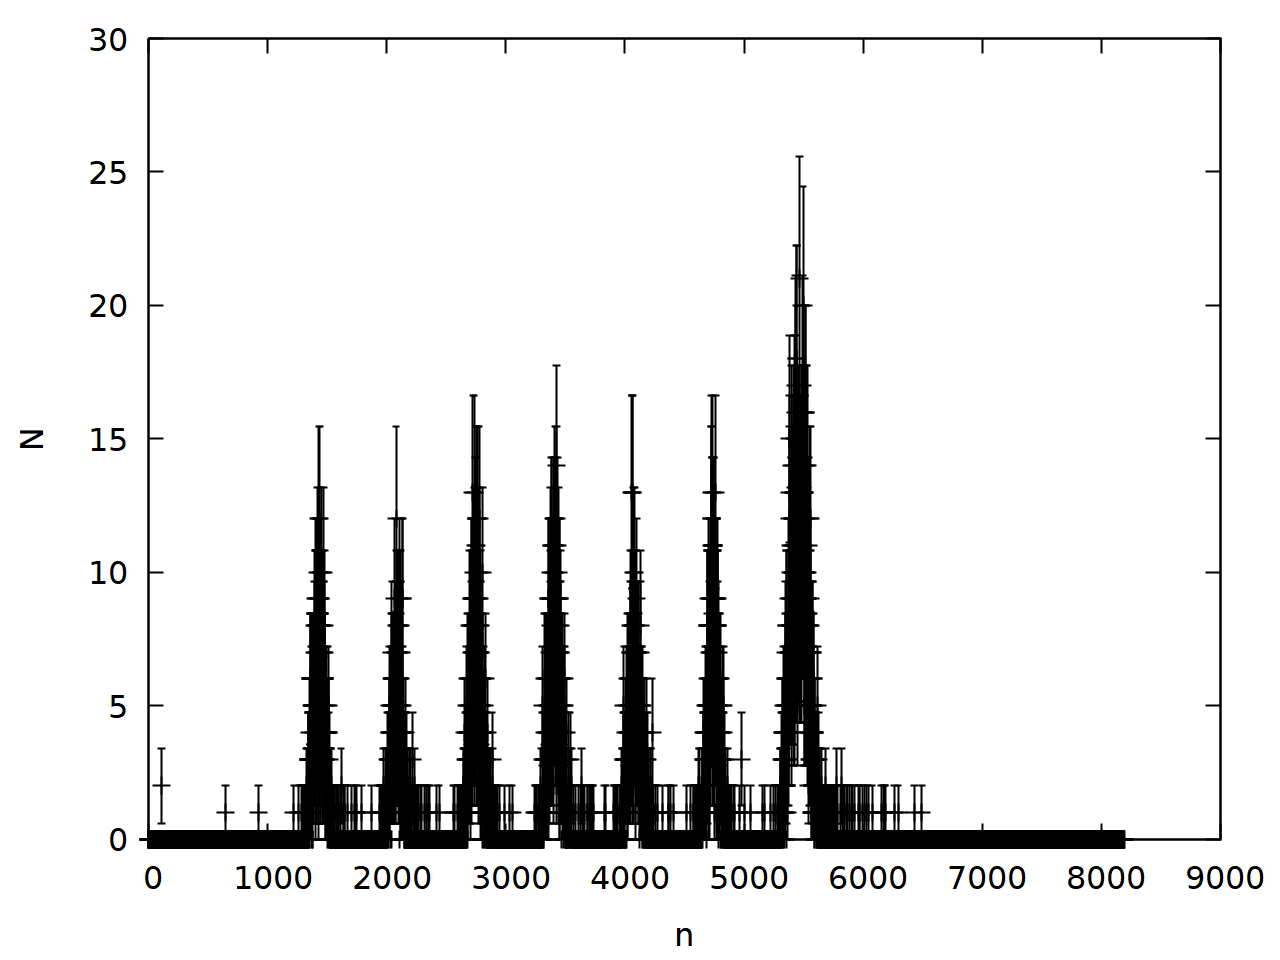
\includegraphics[width=0.7\linewidth]{data/prompt.png}
%\caption{Gemessene Promptkurve}
%\label{fig:prompt}
%\end{figure}

\begin{figure}
\centering
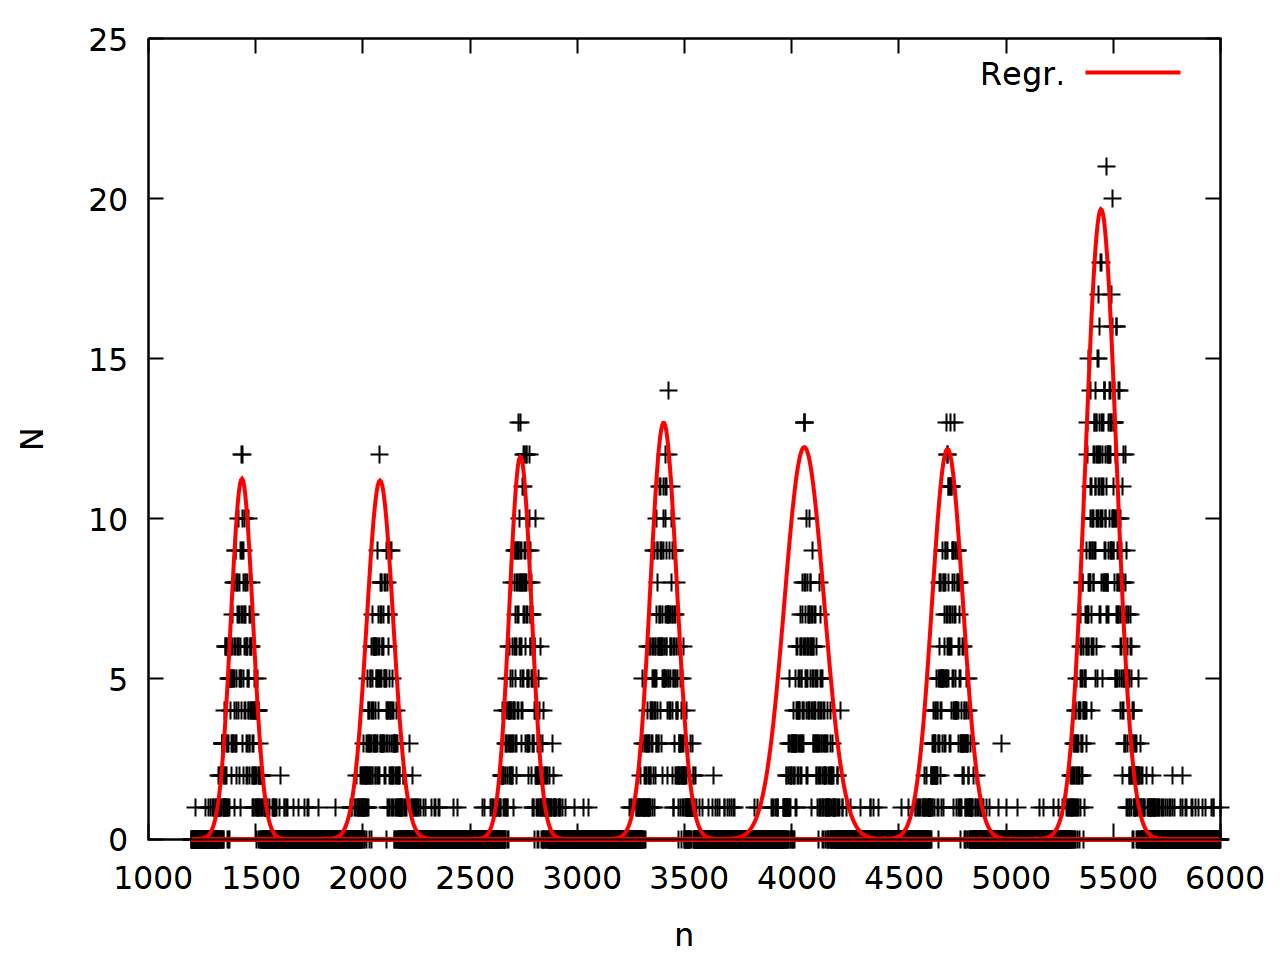
\includegraphics[width=0.7\linewidth]{data/prompt2.png}
\caption{Promptkurve mit Fits}
\label{fig:prompt2}
\end{figure}

\begin{table}
\centering
\caption{Fitergebnisse für die Gausskurven}
\begin{tabular}{cccc}
\toprule
Peak Nr. & a & n & $\sigma$\\
\midrule
6&	19,67&	5443&	72,19\\
5&	12,18&	4727&	72,19\\
4&	12,24&	4059&	92,58\\
3&	13&	3403&	62\\
2&	11,95&	2735&	51,81\\
1&	11,2&	2080&	62\\
0&	11,25&	1436&	51,81\\
\bottomrule
\end{tabular}
\label{tab:prompt}
\end{table}

In Abbildung \ref{fig:prompt2} ist die gemessene Promptkurve zu sehen. An die einzelnen Peaks wird nun jeweils eine Gausskurve \[f(x) = a\exp{\left(-\frac{(x-n)^2}{2\sigma^2}\right)}\]mit Fityk gefittet. Das Ergebnis ist in Tabelle \ref{tab:prompt} aufgelistet (Die Fehler der Fitparameter sind nicht relevant, da später $\sigma$ als Fehler verwendet wird.).\\

Der Abstand der Peaks entspricht jeweils \SI{16}{\nano\second}. Um zu bestimmen, wie vielen Kanälen diese \SI{16}{\nano\second} entsprechen, wird die Position des Peaks über der Peaknummer multipliziert mit \SI{16}{\nano\second} aufgetragen (siehe Abbildung \ref{fig:prompt_time}). Als Fehler der Peakpositionen wird die Standartabweichung $\sigma$ angenommen.  

\begin{figure}
\centering
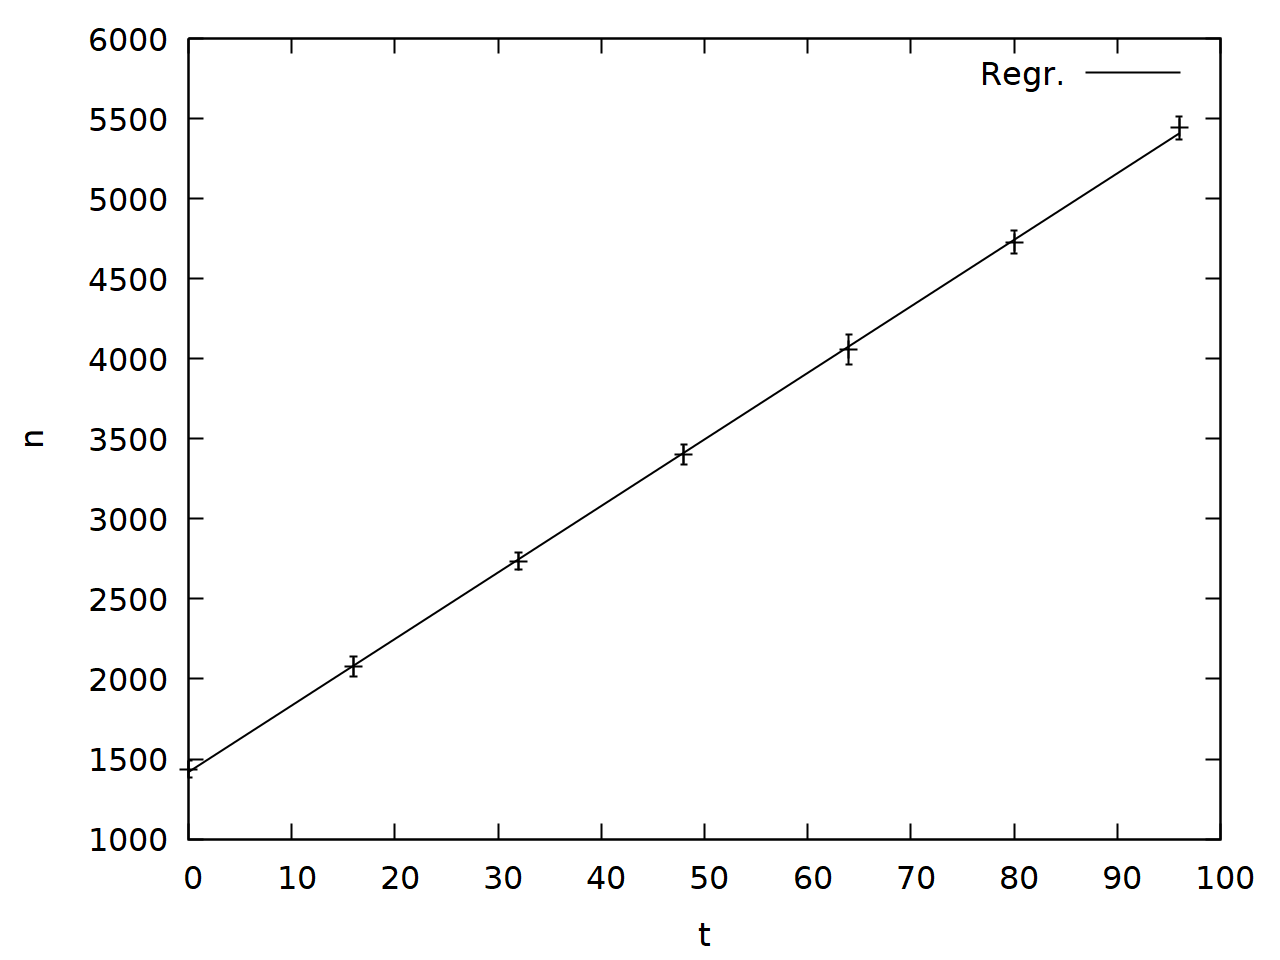
\includegraphics[width=0.7\linewidth]{data/prompt_time.png}
\caption{Positionen der Peaks über der Zeit}
\label{fig:prompt_time}
\end{figure}

Ein linearer Fit $n(t)=a\cdot t + b$ ergibt
\begin{align*}
a &= \SI[separate-uncertainty=true]{41.5 \pm 0.2}{\per\nano\per\second}\\
b &= (1,42 \pm 0,01) \cdot 10^{3}.
\end{align*}
Das bedeutet, dass \SI{1}{\nano\second} 41,5 Kanälen entspricht.\\

Um die Zeitauflösung zu bestimmen wird der Mittelwert (und Standartabweichung) aller $\sigma$ gebildet. Man erhält eine Zeitauflösung von 66 Kanälen bzw. \SI[separate-uncertainty=true]{1.6 \pm 0.3}{\nano\second}.

\subsection{Bestimmung der Lebensdauer}

\begin{figure}[h]
\centering
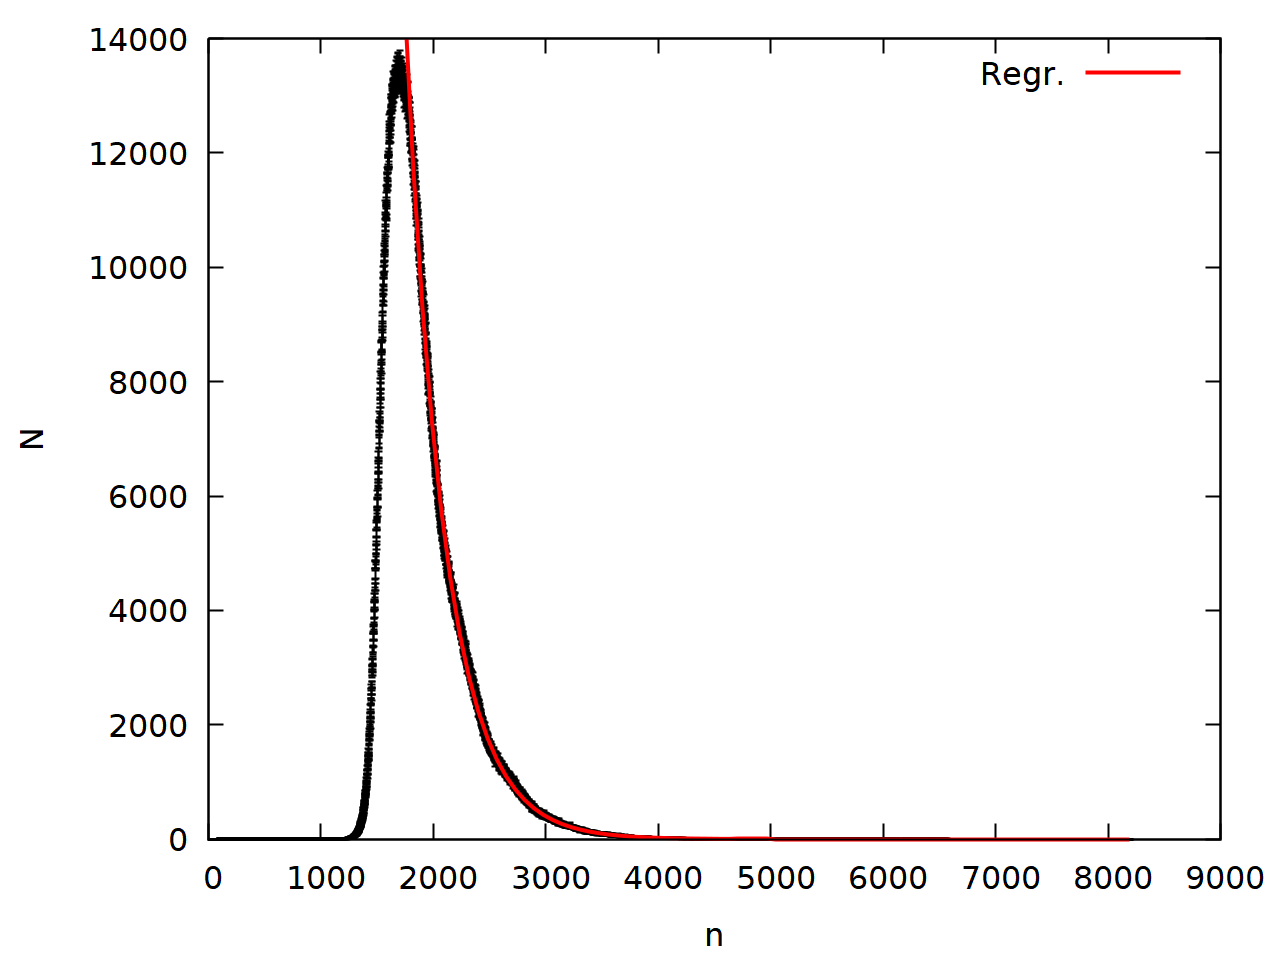
\includegraphics[width=0.7\linewidth]{data/uebernacht.png}
\caption{Ergebnis der Lebensdauermessung}
\label{fig:halflife}
\end{figure}

In Abbildung \ref{fig:halflife} sind die gemessenen Ereignisse über den Kanälen aufgetragen. An diesen Daten wird nun im fallenden Bereich ($n \geq 1750$) ein exponentieller Fit $N(n)=b\cdot e^{-c\cdot (n-1750)}$ durchgeführt (siehe Abbildung \ref{fig:halflife2}). Der Fit ergibt
\begin{align*}
b &= (14,41 \pm 0,02) \cdot 10^3\\
c &= (2,87 \pm 0,002) \cdot 10^{-3} \mathrel{\widehat{=}} (119,2 \pm 0,7)\cdot 10^{-3} \si{\nano\second}^{-1}\\
\end{align*}

Daraus folgt, dass die Halbwertszeit $T_{1/2} = \frac{\ln{2}}{c} = (5,81 \pm 0,03) \si{\nano\second}$ ist. Der Literaturwert liegt bei \SI{6,28}{\nano\second} \cite{cs133}. Der gemessene Wert liegt also in der Nähe des eigentlichen Wertes, allerdings um etwa 15 Standartabweichungen entfernt. Die kleinen Fehler kommen vor allem von den kleinen Fitfehlern. In den Abbildungen \ref{fig:prompt_time} und \ref{fig:halflife2} kann man aber auch erkennen, dass die Fits sehr genau sind. Demzufolge sollten diese auch kleine Fehler haben. Wir gehen deswegen davon aus, dass die Abweichung nicht durch die Auswertung zu erklären sind, sondern durch einen systematischen Fehler im Versuchsaufbau. Dies müsste durch einen Effekt geschehen, der den Abfall der Exponentialfunktion größer macht, also kleinere Zeiten häufiger auftreten als größere. Es wird vermutet, dass das durch zufällige Ereignisse entsteht. Tritt ein zufälliges Ereignis vor dem Stopsignal auf (aber auch innerhalb der Koinzidenz der beiden Slow-Signale), so wird dieses Signal als Stopsignal interpretiert und somit eine kleinere Zeit gemessen. Dieser Effekt ist natürlich bei höheren Zeitabständen größer, da die Wahrscheinlichkeit für ein zufälliges Ereignis zwischen Start- und Stopsignal dann größer ist. Somit verschiebt sich die Kurve zu kleineren Energien und es ergibt sich eine Exponentialfunktion mit stärkerem Abfall und kleinerer Halbwertszeit. 

\begin{figure}[h]
\centering
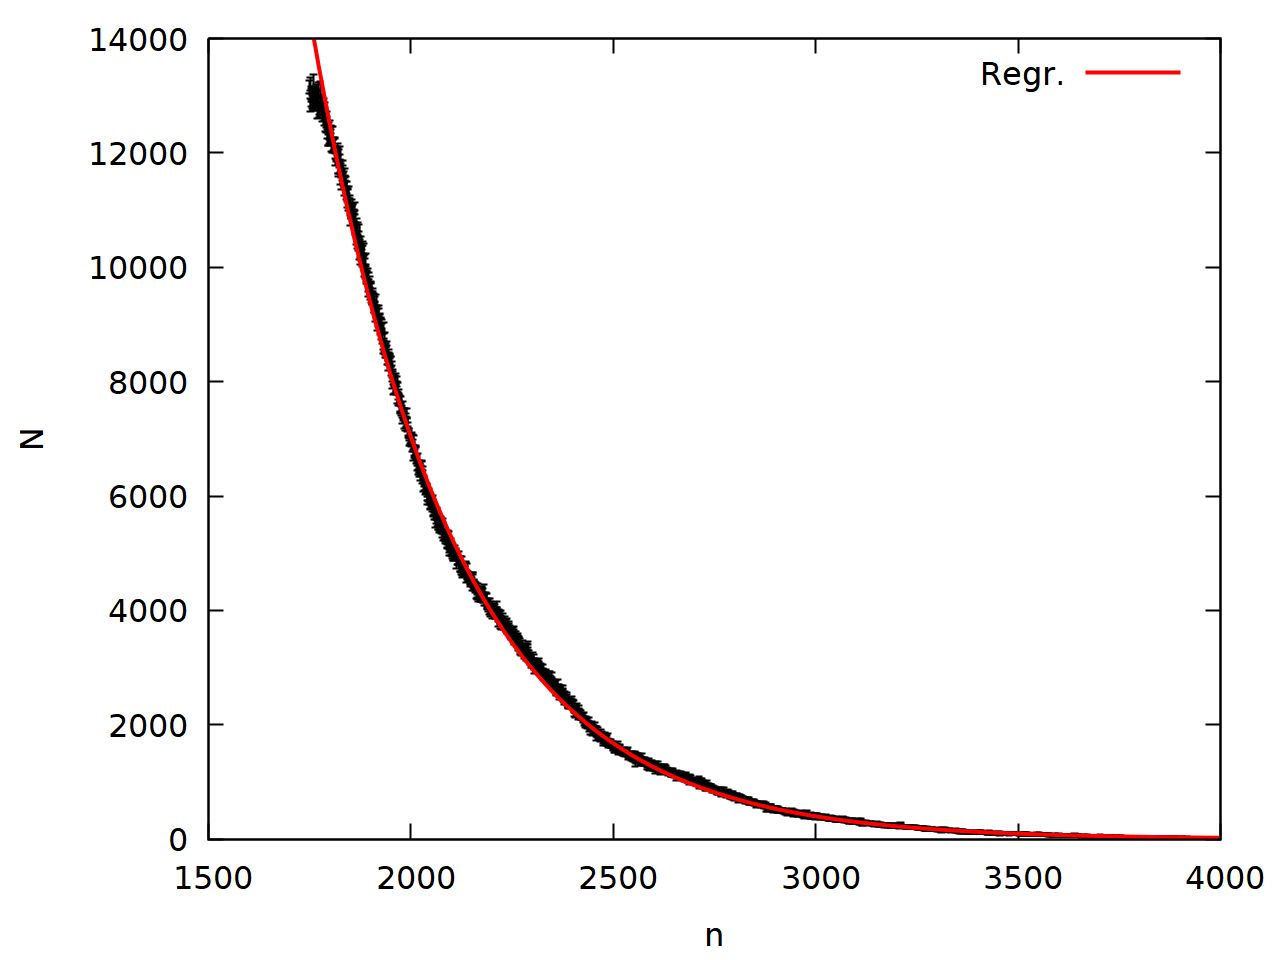
\includegraphics[width=0.7\linewidth]{data/uebernacht2.png}
\caption{Exponentieller Fit an die Lebensdauermessung}
\label{fig:halflife2}
\end{figure}
